\documentclass{article}
\usepackage[utf8]{inputenc}
\usepackage{graphicx}
\graphicspath{ {assets/} }

\title{Poročilo}
\author{Mai Praskalo in Žan Gostič}
\date{November 2022}

\begin{document}

\maketitle

\section{Osnovne informacije}

\begin{itemize}
    \item \textbf{Naslov projekta}: Primerjalnik cen izdelkov
    \item \textbf{Člana skupine}: Mai Praskalo, Žan Gostič
    \item \textbf{Ogrodje in razvojno okolje}: Java, KumuluzEE
    \item  \textbf{Kratek opis projekta}: Aplikacija bo omogočila prikaz cen različnih izdelkov in razlike v cenah le teh med trgovinami. Poleg tega bo omogočala tudi generiranje najcenejše košarice za izbrane izdelke, izračun košarice priljubljenih izdelkov in shranjevanje košarice izbranih izdelkov.
\end{itemize}
\pagebreak
\section{Shema arhitekture in interakcij med storitvami}

\begin{figure}[h]
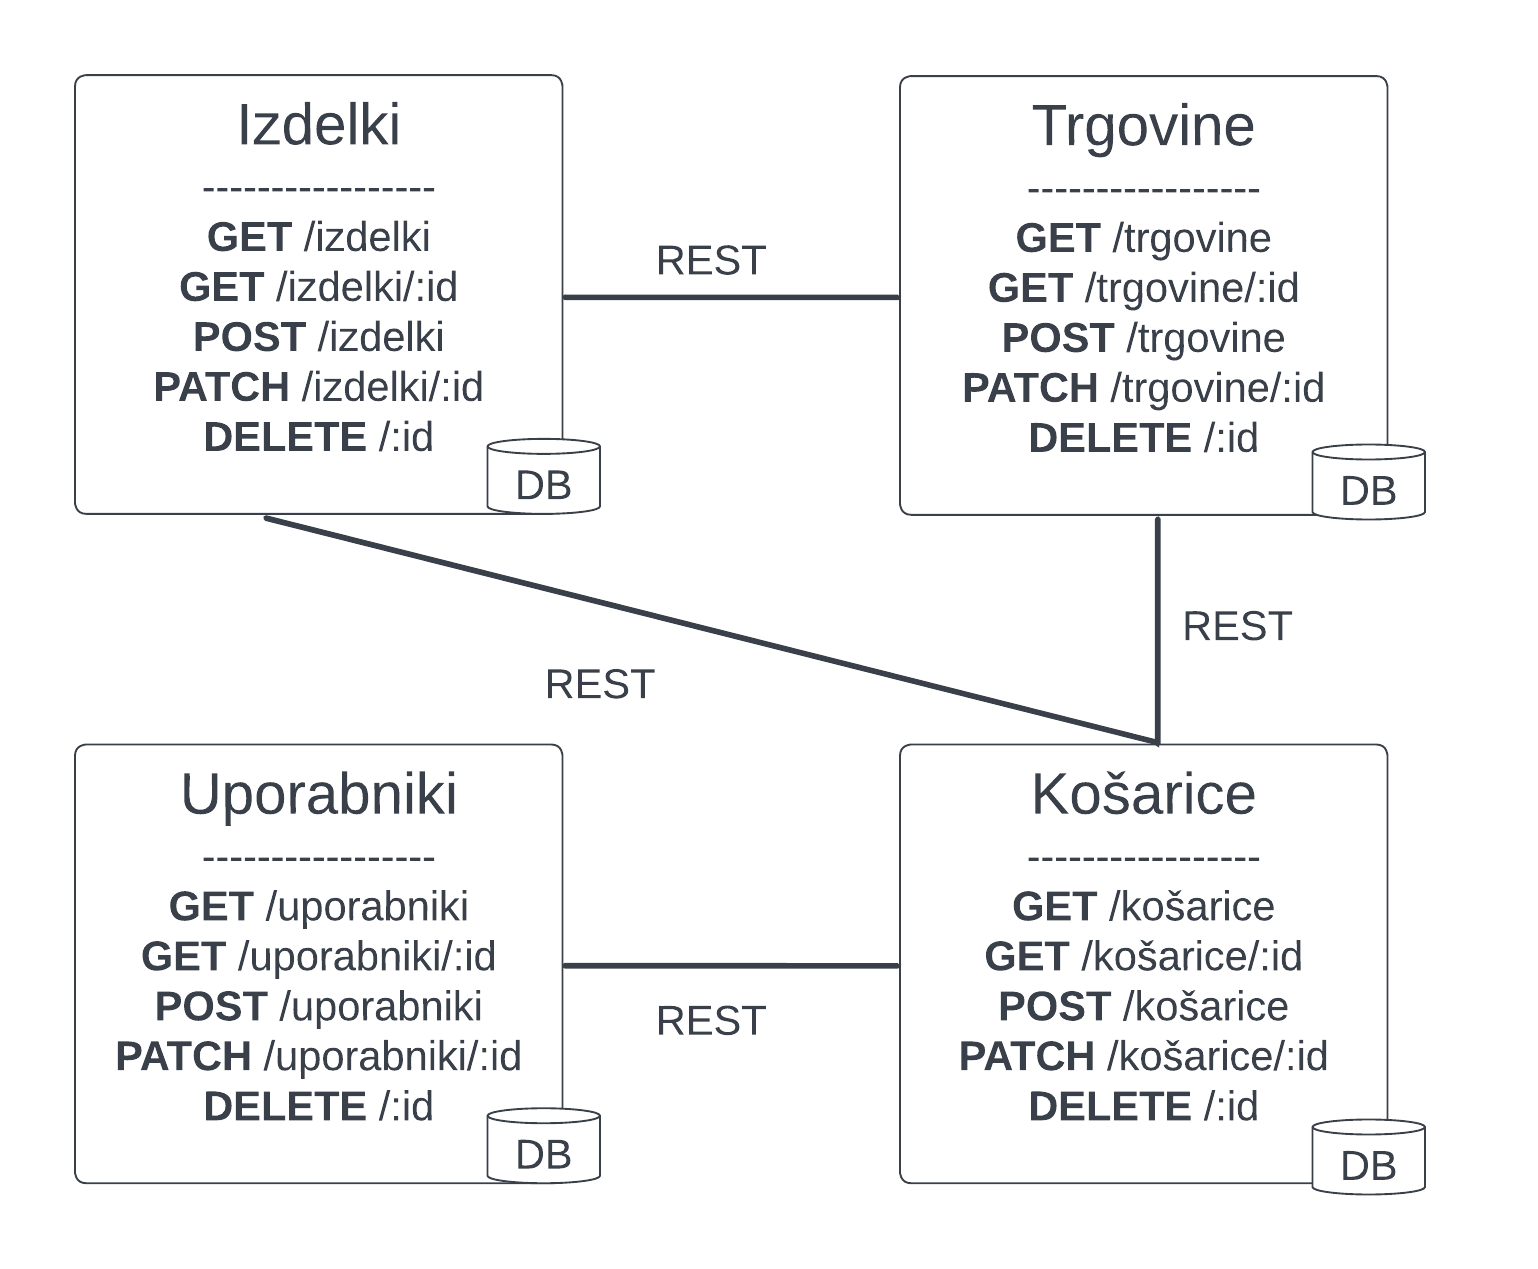
\includegraphics{schema.png}
\centering
\end{figure}

\section{Funkcionalnosti}
\subsection{Izdelki}
Storitev, ki je namenjena za upravljanje z izdelki.

\begin{itemize}
    \item Pridobitev vseh izdelkov
    \item Pridobitev posamičnih izdelkov
    \item Dodajanje izdelka
    \item Posodobitev izdelka
    \item Brisanje izdelka
\end{itemize}

\subsection{Trgovine}
Storitev, ki je namenjena za upravljanje s trgovinami.

\begin{itemize}
    \item Pridobitev vseh trgovin
    \item Pridobitev posamičnih trgovin
    \item Dodajanje trgovin
    \item Posodobitev trgovin
    \item Brisanje trgovin
\end{itemize}

\begin{itemize}
    \item Pridobitev vseh trgovin
    \item Pridobitev posamičnih trgovin
    \item Dodajanje trgovin
    \item Posodobitev trgovin
    \item Brisanje trgovin
\end{itemize}

\subsection{Uporabniki}
\begin{itemize}
    \item Pridobitev vseh košaric
    \item Pridobitev posamičnih košaric
    \item Dodajanje košarice
    \item Posodobitev košarice
    \item Brisanje košarice
\end{itemize}

\section{Primeri uporabe}
\begin{itemize}
    \item Primerjava cen izdelkov med trgovinami.
    \item Shranjevanje košarice izdelkov.
    \item Generiranje najcenejše košarice glede na izbrane izdelke.
    \item Izračun košarice najbolj priljubljenih izdelkov uporabnikov.
\end{itemize}
\end{document}
